\documentclass[a4paper,11pt,uplatex]{jsbook}
%\usepackage{fancyhdr}
\setlength{\footskip}{16pt}
\usepackage{amsmath}
\usepackage[dvipdfmx]{graphicx}
\usepackage[dvipdfmx]{color}
%\usepackage{pagecolor}[white]
\usepackage{amsmath,amssymb}
%\usepackage[top=3cm, bottom=3cm, left=3cm, right=3cm]{geometry}
\usepackage{braket}
\usepackage{bm}
\numberwithin{equation}{section}
\usepackage{mathrsfs}
\usepackage{siunitx}
\usepackage{physics}
\usepackage[dvipdfmx]{graphicx}
\usepackage[compat=1.1.0]{tikz-feynhand}
\usepackage{caption}
\usepackage{subcaption}
%\usepackage{cleveref}
\usepackage{float}
\usepackage{multicol}
\setlength{\columnsep}{15mm}
%\usepackage[style=phys,articletitle=false,biblabel=brackets,chaptertitle=false,pageranges=false]{biblatex}
%\usepackage[style=phys]{biblatex}
\usepackage[dvipdfmx]{hyperref}
\usepackage{url}
\usepackage{pxjahyper}
\usepackage{bookmark}
%\usepackage[backref]{hyperref}
\setcounter{tocdepth}{3}
\setlength{\parindent}{2em}
\def\vector#1{\mbox{\boldmath $#1$}}
\def\slash#1{\not\!#1}
\def\slashb#1{\not\!\!#1}
\def\delsla{\not\!\partial}
%\usepackage[dvipdfmx]{xcolor}


\hypersetup{
 setpagesize=false,
 bookmarksnumbered=true,%
 bookmarksopen=true,%
 colorlinks=true,%
 linkcolor=black,
 citecolor=red,
 urlcolor=black,
}
%backreferenceのカスタマイズ. "Back to p.3"のように表示する.
%\renewcommand*{\backref}[1]{(p.#1へ戻る)}
%\newcommand{\backtoc}{\hyperlink{toc}{[目次へ]}}
\newcommand{\backtoc}{\texorpdfstring{\protect\hyperlink{toc}{\hspace{5pt} \scriptsize [目次へ]}}{}}
\newcommand{\mychapter}[1]{\chapter[#1]{#1\backtoc}}
\newcommand{\mysection}[1]{\section[#1]{#1\backtoc}}
\newcommand{\mysubsection}[1]{\subsection[#1]{#1\backtoc}}

% 数式
%\usepackage{amsmath,amsfonts}
%\usepackage{bm}
%\usepackage{physics}
% 画像
%\usepackage[dvipdfmx]{graphicx}
%\usepackage[dvipdfmx,colorlinks=true,linkcolor=blue]{hyperref}
%\usepackage{pxjahyper}

\begin{document}


\chapter{MAMIにおける測定手法}
この章の目的は、実験に用いた装置の性能や仕様、およびセットアップの手法を説明することである。
まず加速器とMAMIの概要を示し、高品質のアンジュレータ放射光を得るための制御方法を説明する。
次に、電子ビームエネルギー測定に不可欠な分光光学系の構成とアラインメント方法を示す。
最後に、ビームタイム中のデータ取得の手順を示す。
\section{装置とセットアップ}
\subsection{マインツマイクロトロン(MAMI)}\label{sec:MAMI}
MAinz MIcrotron~(MAMI)はドイツ、マインツ大学が所有する連続電子線加速器施設である。最大エネルギー1508 MeVの電子ビームを供給する
3台のRTM(Race Track Microtron)および1台のHDSM(Harmonic Double Sided Micrtron)から構成される。
MAMIのフロアマップを図\ref{fig:MAMI}に、主なパラメータを表\ref{MAMI}に示した。
ハイパー核生成実験ではHDSMを用いて最大エネルギーの1508 MeVの電子ビームを供給する。

スペクトロメータ較正実験では、RTM3までで加速された180 MeVから210 MeVまでの電子ビームを用いる。
\begin{figure}[H]
  \centering
  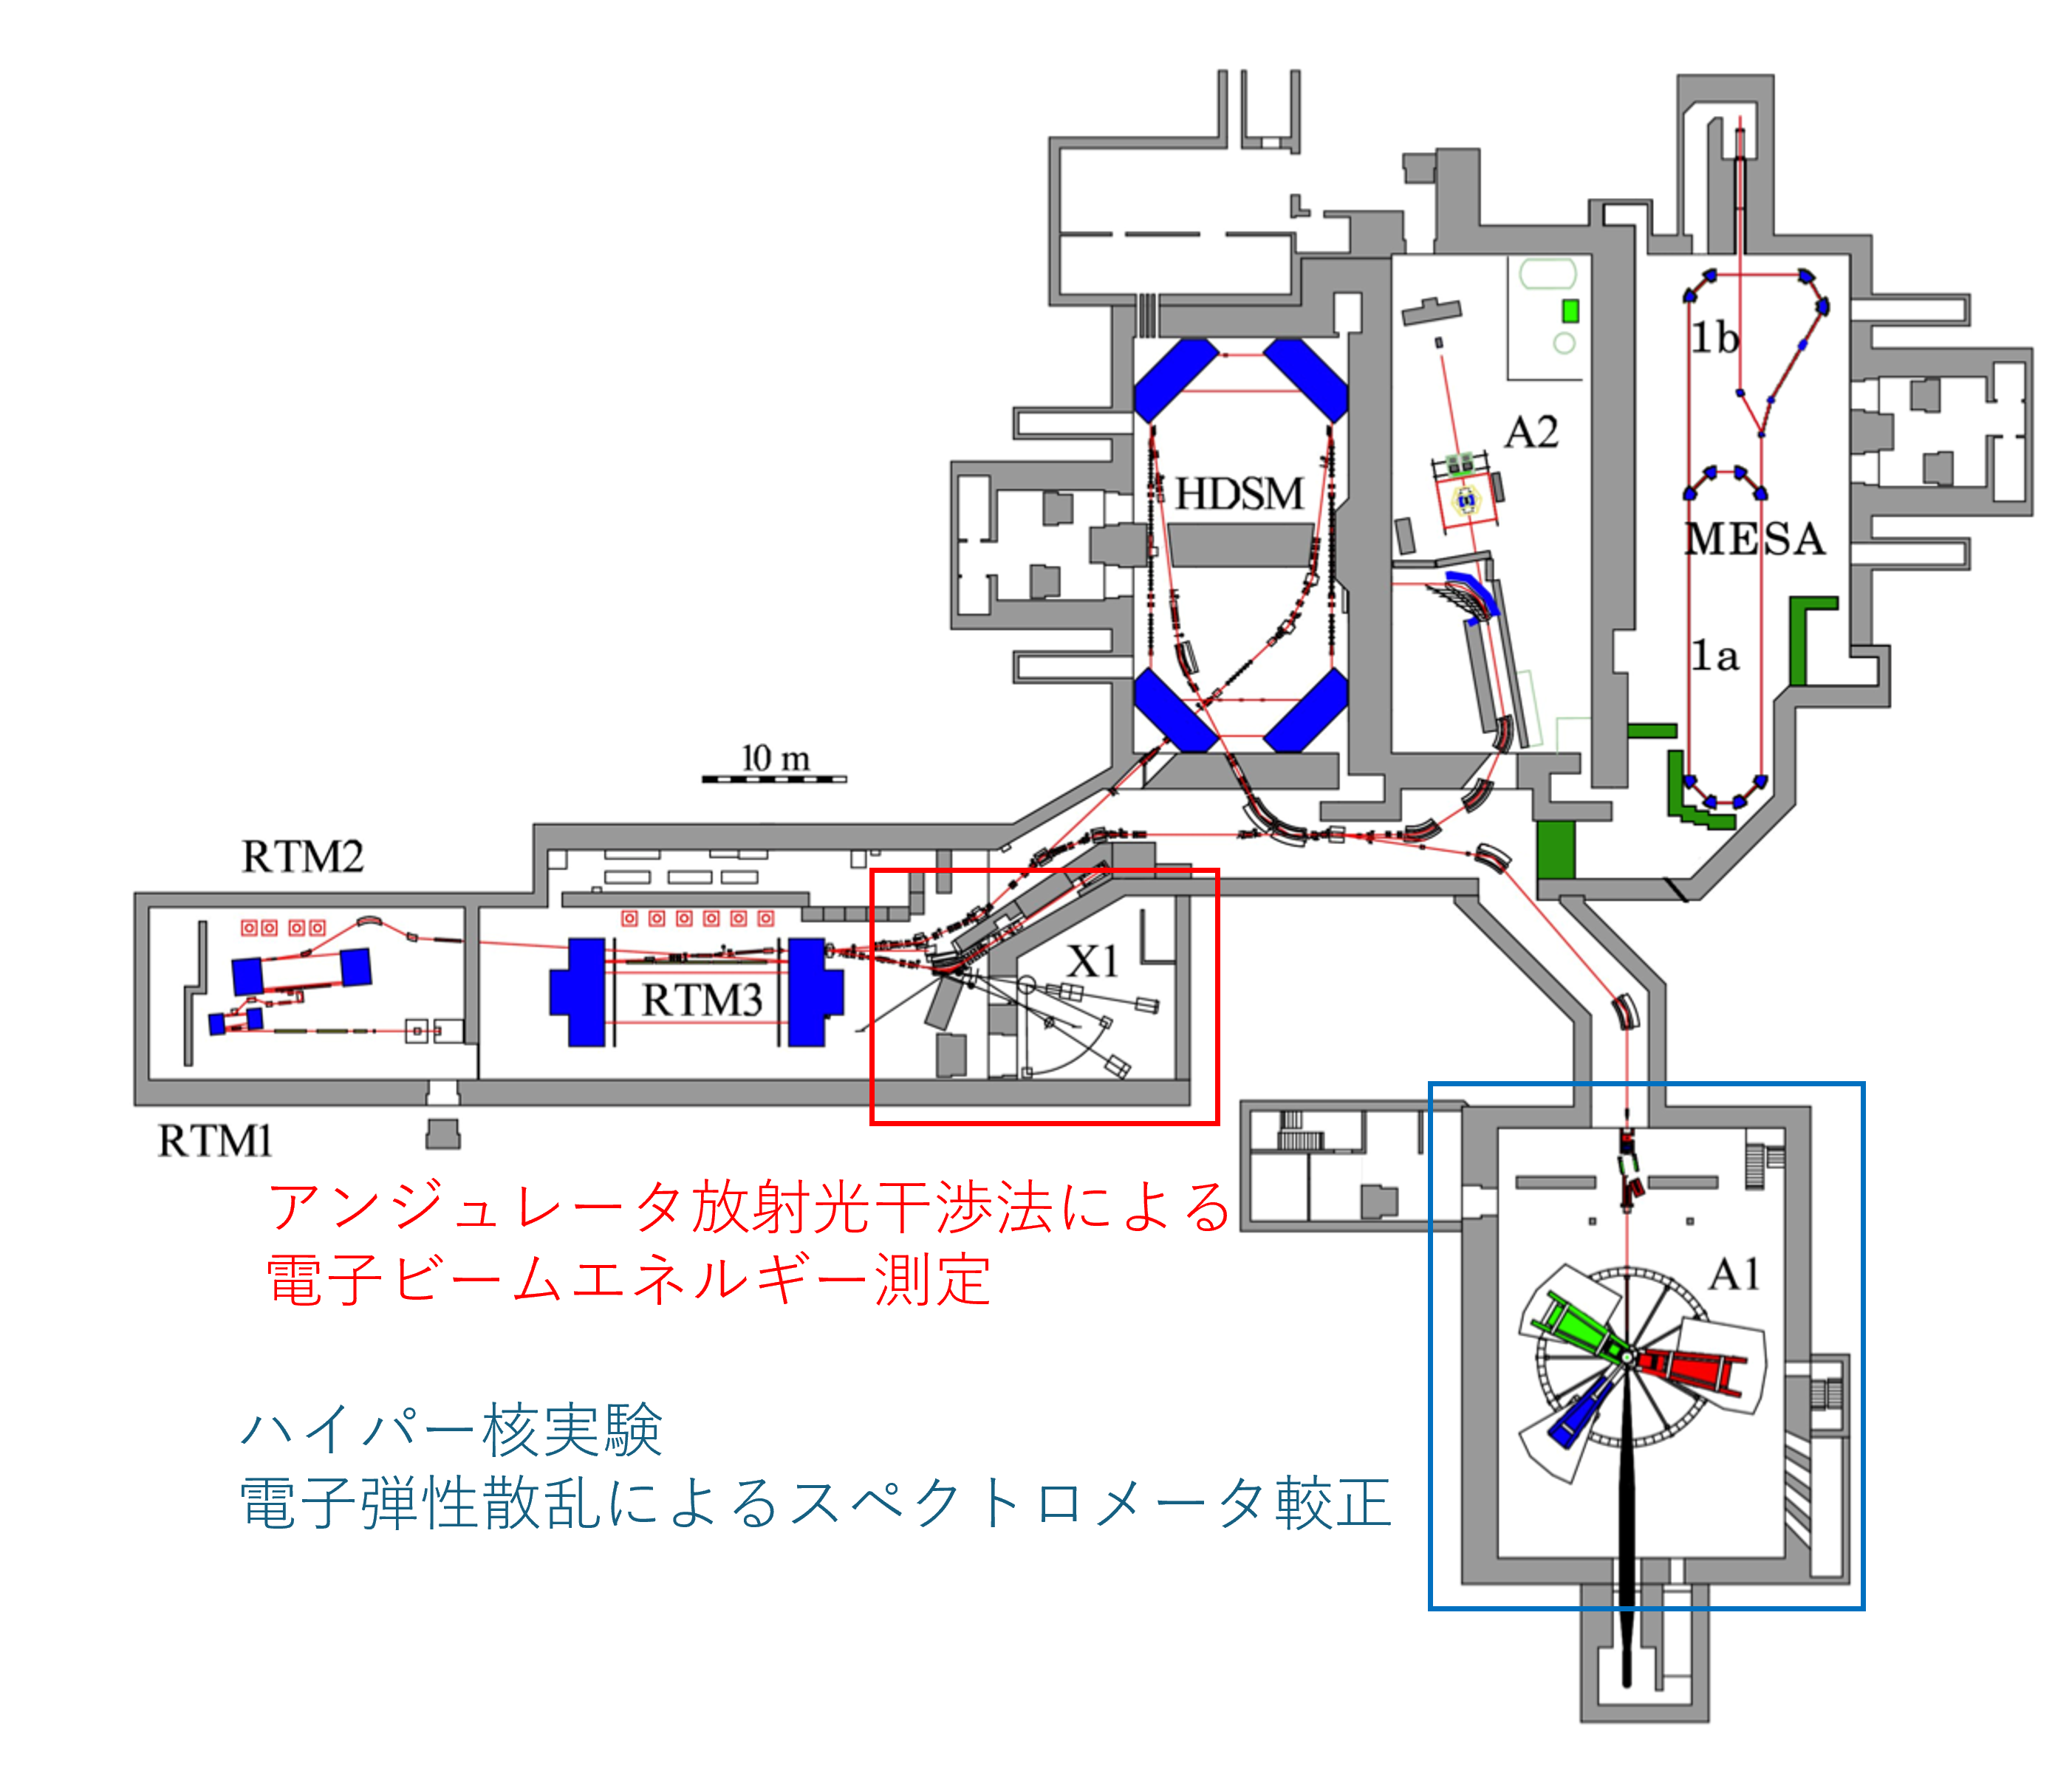
\includegraphics[width=0.8\linewidth]{image/3-MAMI.png}\\
  \caption[MAMIのフロアマップ]{MAMIのフロアマップ。RTM1,RTM2,RTM3で加速された電子ビームはX1ホール(赤)またはA1ホール(青)に供給される。X1ホールではアンジュレータ放射光干渉法による電子ビームエネルギー測定を行う。またA1ホールでは電子弾性散乱実験を行う。}
  \label{fig:MAMI}
\end{figure}
\begin{table}[H]
  \caption{MAMIの主要パラメータ}\label{MAMI}
  \centering
  \begin{tabular}{c||cc}
    \hline
     &RTM3 & HDSM \\
    \hline
    最大エネルギー & 855.1 MeV & 1508 MeV \\
    最大強度 & 100 $\mu$A & 100 $\mu$A \\
    周回数 & 90 & 43 \\
    偏光磁石の磁場 &1.28 T & 0.95 - 1.53 T\\
    周波数 & 2.45 GHz & 2.45 / 4.9 GHz \\
    エネルギー幅 & 13 keV & 110 keV \\
    水平方向エミッタンス & 13 $\pi$ $\mu$m mrad & 27 $\pi$ $\mu$m mrad \\
    垂直方向エミッタンス & 0.84 $\pi$ $\mu$m mrad & 1.2 $\pi$ $\mu$m mrad\\
    \hline
  \end{tabular}
\end{table}
ここでは本研究で用いる200 MeV領域の電子ビームに注目し、RTM3における加速機構を説明する。
図\ref{RTM3}にRTM3の模式図を示した。2つの180$^\circ$偏向電磁石の間には線形加速器(LINAC)が設置されている。
前段の加速器で180 MeVまで加速され入射された電子はLINACで加速されるごとにおよそ15 MeVエネルギーを得る。加速されると偏向電磁石での軌道半径が大きくなり、
一つ外側の周回軌道を通り再びLINACで加速を受ける。このようにして電子は周回軌道を繰り返し、最終的に最大で855 MeVまで加速されて実験ホールに供給される。
周回軌道の途中にはビーム取り出しのためのキッカーマグネットが設置されており、このキッカーマグネットをどの軌道に設置するかによって周回回数を調節し、供給するエネルギーを決定する。
\begin{figure}[h]
  \centering
  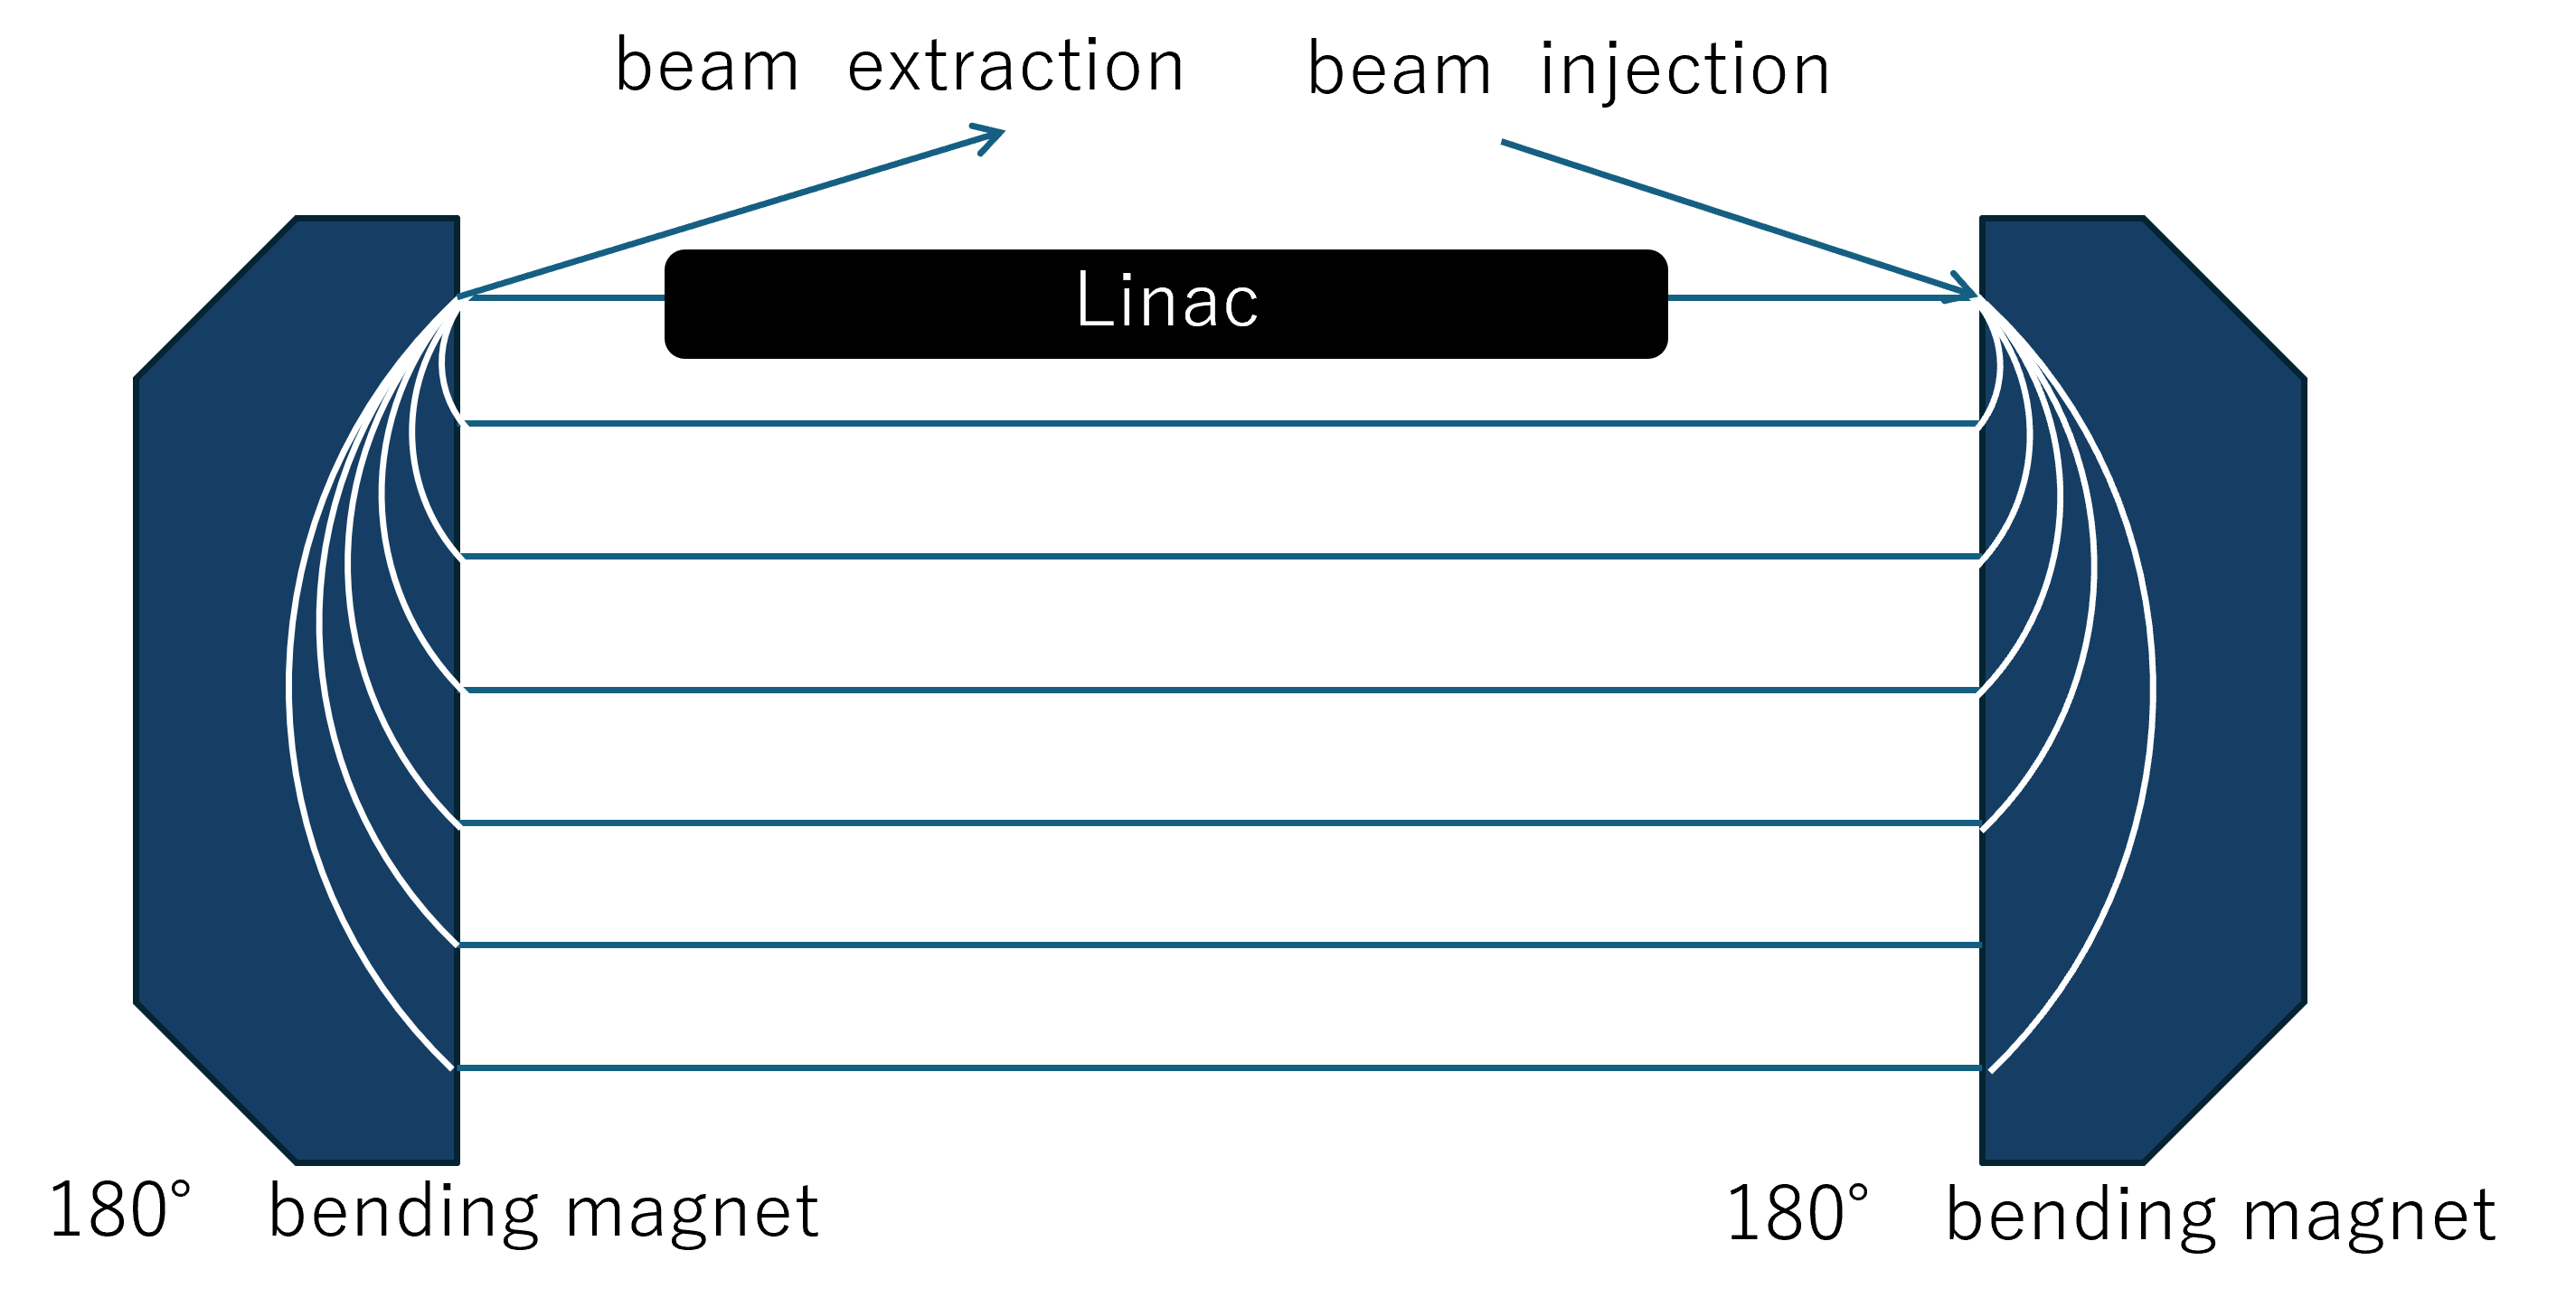
\includegraphics[width=0.8\linewidth]{image/3-RTM.png}\\
  \caption[RTM3の模式図]{RTM3の模式図。前段のRTM2で180 MeVまで加速された電子ビームは180$^\circ$偏向電磁石でもっとも軌道半径の小さい周回軌道に入る。
  1周してLINACで加速されるごとに15 MeVずつエネルギーが増加し、これに伴い軌道半径が大きくなり、一つ外側の周回軌道を通り再びLINACで加速を受ける。
  軌道中に設置したキッカーマグネットによって周回軌道からずれビーム取り出しビームラインに供給される。}
  \label{RTM3}
\end{figure}

RTM3には計90周の周回軌道があり、1周毎に15~MeVずつ加速されるが、このうち73週目の軌道にビームポジションモニタが設置されている。
RTM3の180$^\circ$偏向電磁石中での軌道半径$R_{73}$を測定し、得られたビームエネルギー$E_{73}$からMAMIで確立された粒子トラッキングシステムPTRACE\cite{ratschow}を用いて$n$周目のビームエネルギー$E_n$を外挿して求める。
180$^\circ$偏向電磁石の磁場はNMRを用いて$10^{-4}$の精度で測定されている。またPTRACEの計算で生じる誤差が0.1~mm、ビームパイプの位置決定精度が0.43~mmと見積もられており、
これらの誤差を考慮して$E_{73}\sim 727~$MeVにおけるエネルギーの誤差は$\delta E_{73} =120$~keVと見積もられている\cite{jankowiak}。
$E_{73}$から他の周回軌道のビームエネルギー$E_n$をPTRACEで外挿した結果、$E_n$の誤差は一律で$\delta E_n$ =160~keVと見積もられている\cite{herter}。

RTM3の直後には供給するビームラインを選ぶための偏向電磁石が設置されており極性をレバーで変えることで、アンジュレータ放射光干渉法による電子ビームエネルギー測定を行うX1ホールと、電子弾性散乱によるスペクトロメータ較正を行うA1ホールにビームを供給するモードを切り替えることができる。

\subsubsection{X1ホール}
電子ビームエネルギー測定を行うホールBとX1ホールの構成を図\ref{X1}, \ref{X1-2}に示す。
\begin{figure}[H]
  \centering
  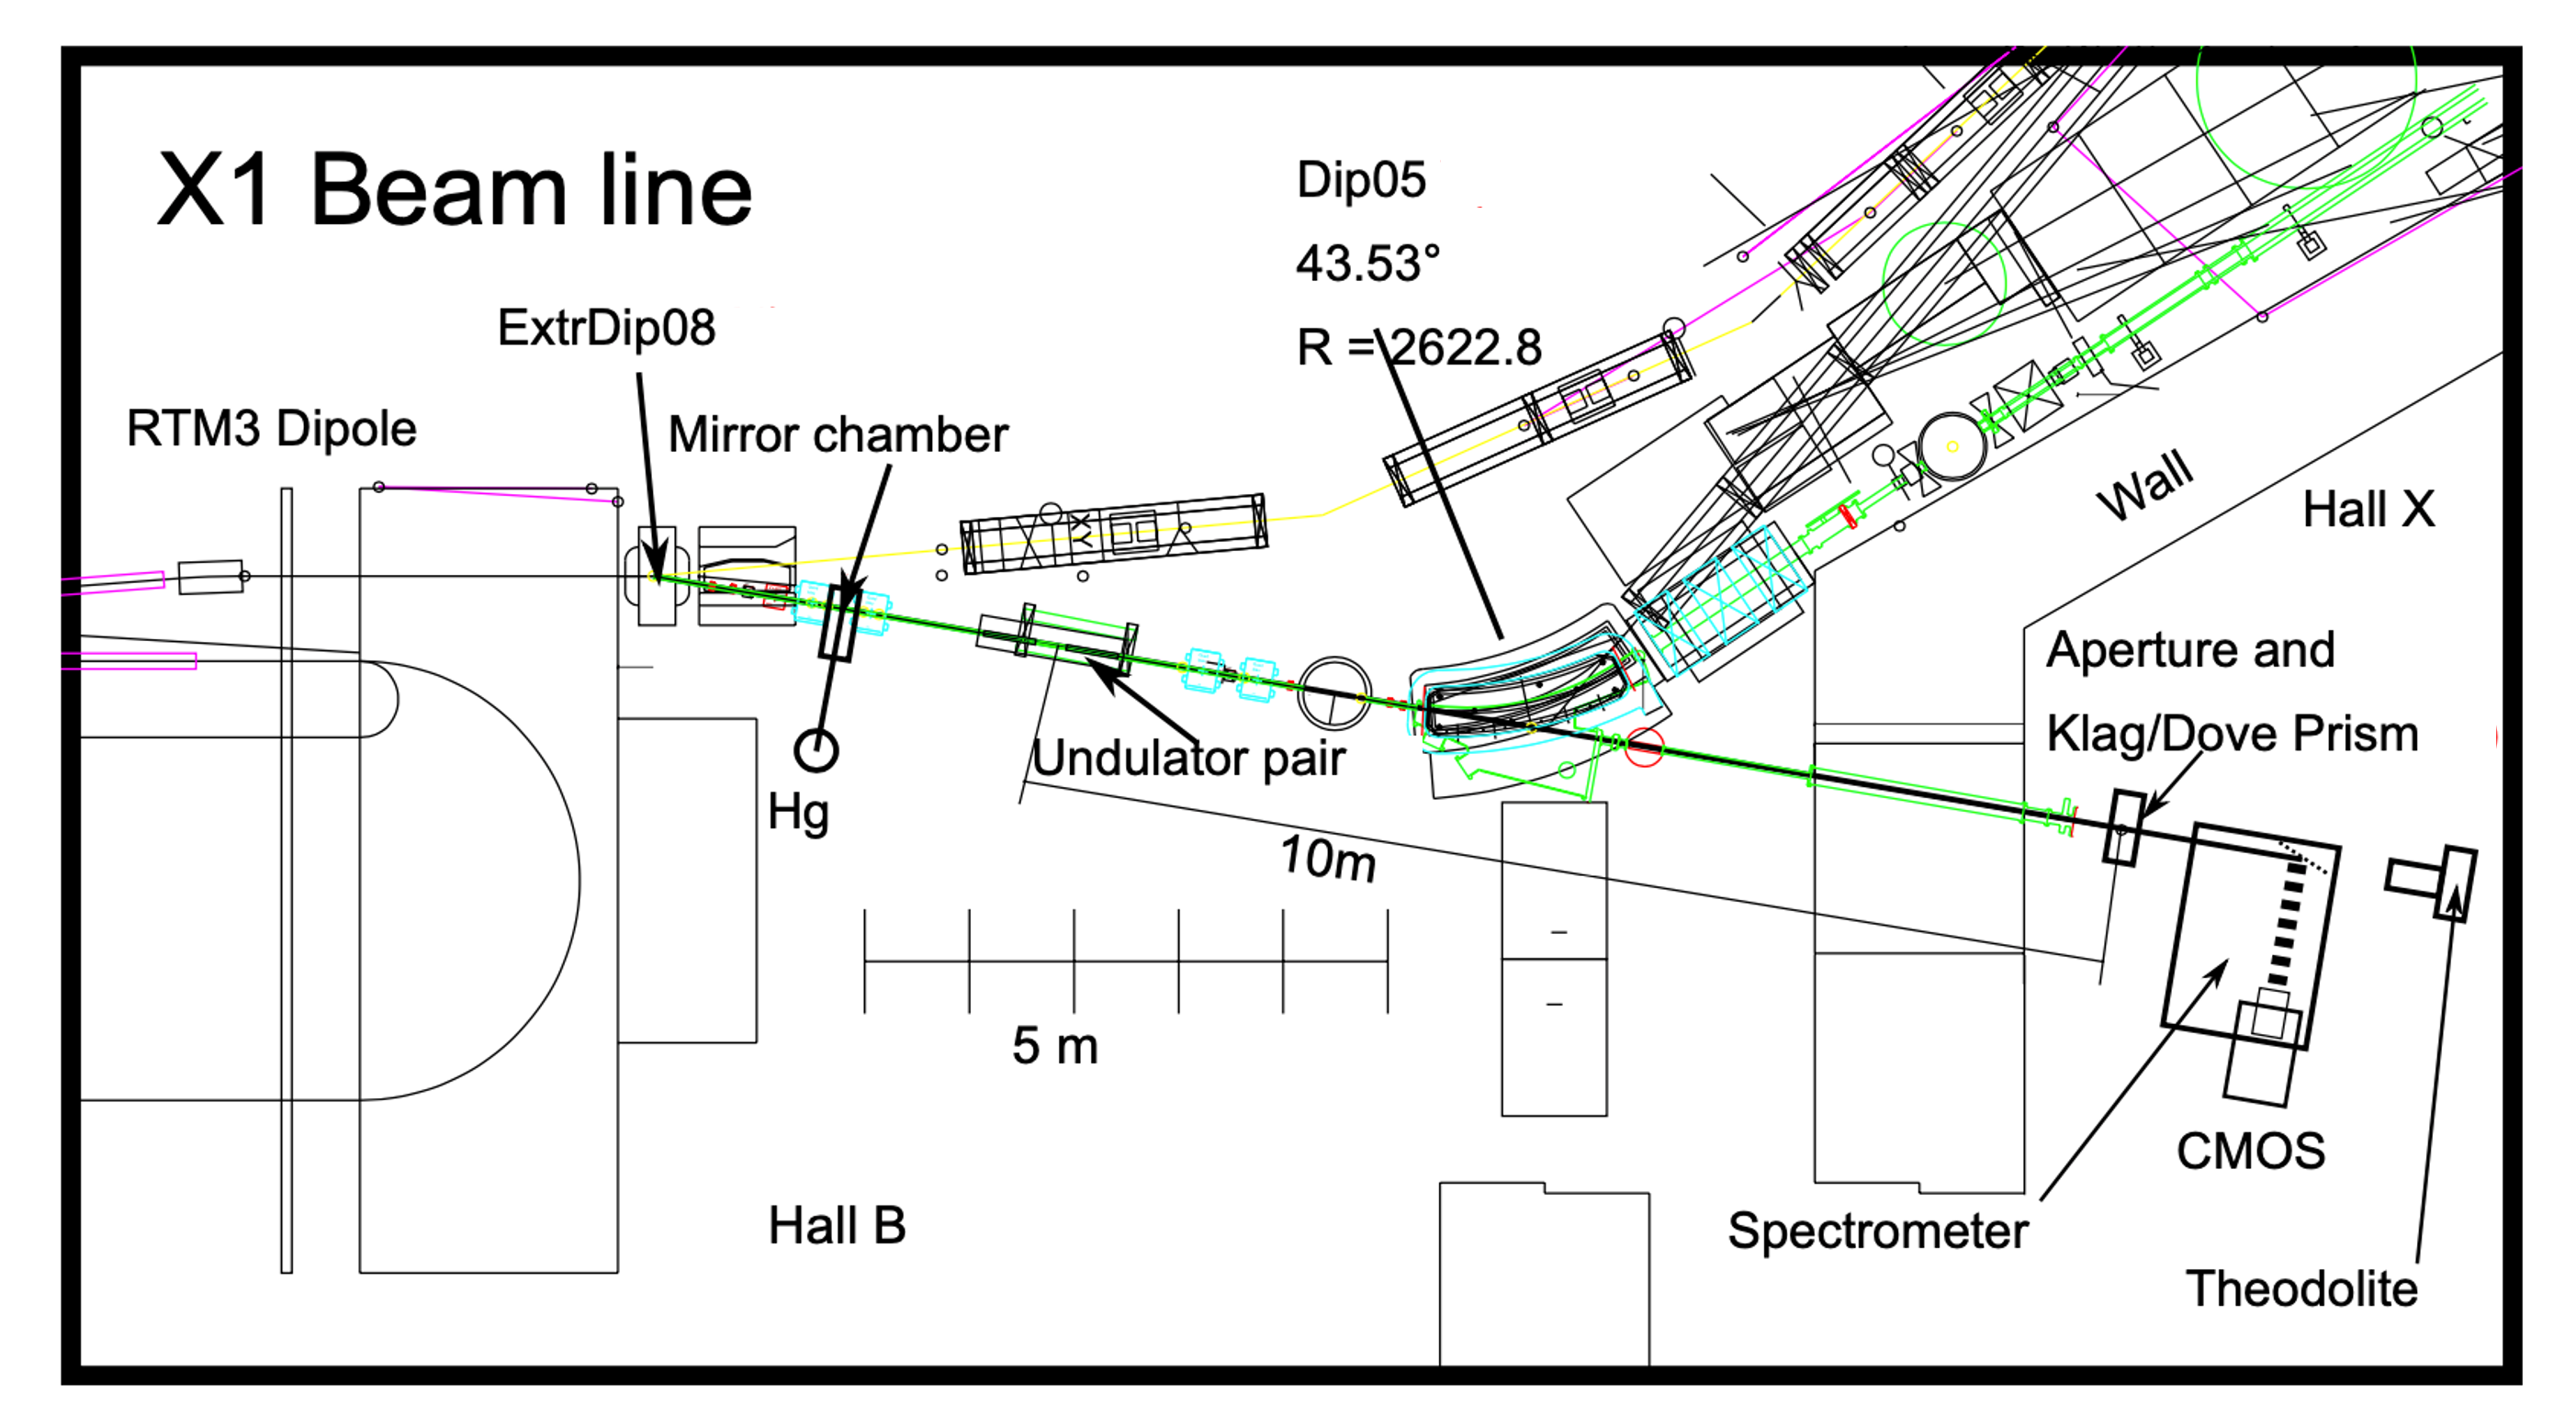
\includegraphics[width=\linewidth]{image/3-X1.png}\\
  \caption[ホールBとX1ホールの模式図]{ホールBとX1ホールの模式図。電子ビームは図の左のRTM3側から供給される。RTM3偏向電磁石の直後にある一つ目の偏向電磁石では電子ビームを供給するビームラインを選択する。
  電子ビームエネルギー測定をおこなうときには電子ビームは図の下側のビームラインへ供給される。四重極電磁石(Q1,Q2)の間にはミラーボックスを設置し
  光学系の較正用のレーザー光をビームラインに導く。Q2の下流にアンジュレータを設置し、ここで放射光を発生させる。アンジュレータの下流には更に2つの四重極電磁石Q3,Q4、および偏向電磁石が設置されている。
  偏向電磁石によって電子ビームはビームダンプへ導かれ、放射光のみを観測する光学系に導くことができる。コンクリート壁を隔ててX1ホールに光学系を設置し放射光のデータ取得を行うほか、更に下流にはアラインメント用のセオドライトを設置する}
  \label{X1}
\end{figure}
\begin{figure}[H]
  \centering
  \includegraphics[width=\linewidth]{image/3-HallB.png}\\
  \caption[ホールBの写真]{ホールBのビームラインを上から撮影した画像。図\ref{X1}の模式図のQ1からビームダンプへの偏向電磁石までが見えている。}
  \label{X1-2}
\end{figure}
電子ビームの軌道を調整するための電磁石がRTM3に設置されており、水平方向、垂直方向のビーム位置を調整する。
RTMの直後にはビームライン選択用の偏向電磁石が設置されている。更に下流には四重極電磁石が2つ(Q1,Q2)設置されており、その間にミラーボックスが設置されている。
Q2の下流にアンジュレータを2台設置する。その下流に更に2台の四重極電磁石(Q3,Q4)が設置されている。
4台の四重極電磁石はアラインメントの基準となるほか、ビーム調整時にも利用するが、測定を行う際には原則利用しない。
その下流には偏向電磁石が設置されており、電子ビームをビームダンプに導くことができる。これにより放射光のみをコンクリート壁に通したビームパイプを通じてX1ホールに導くことができる。
X1ホールには光学系が設置されており、放射光を観測する。アンジュレータから光学系まではおよそ10 mの距離がある。更にその下流側にはアラインメント用のセオドライトが設置されている。

またホールBのビームライン上には光学系の較正用の水銀灯や青色レーザー、ビームライン内の可動式ミラーが設置されている。
水銀灯や青色レーザーによる較正を行う際にはミラーボックス内のミラーをビームライン中心に移動させることで水銀灯や青色レーザーを光学系に供給することができる。
\begin{figure}[H]
  \centering
  \includegraphics[width=0.5\linewidth]{image/3-mirrorbox.png}\\
  \caption[ミラーボックスの写真]{ホールB内に設置されたミラーボックスを真上から撮影した画像。ビームタイム中は蓋がされており、遠隔でモーターを駆動することで
  ミラーを移動させる。写真では電子ビームを供給するモードの状態になっており、電子軌道からミラーが外れている。
  水銀灯による較正を行う際にはミラーが電子軌道に挿入され、図の左から入射する水銀灯の光をビームラインに平行にX1ホールに供給できる}
  \label{mirrorbox}
\end{figure}
\subsubsection{ビーム調整}
まずルミノシティモニタを用いてフェイントビームの位置を目測で調整する。この時の精度は1~mm間隔のグリッドの1/10として100~$\mu$m と見積もられる。
\begin{figure}[H]
  \centering
  \includegraphics[width=0.6\linewidth]{image/3-beamtune.png}\\
  \caption[ルミノシティモニタ]{ルミノシティモニタでのフェイントビームの照射領域。このモニタでビーム位置を目測しながらビーム調整用の電磁石の電流値を調整する。グリッドの間隔は1~mmである。}
  \label{luminosity}
\end{figure}

続いて、ビーム強度を5 $\si{\mu}\text{A}$に上げつつホールB内の放射線モニターで測定される放射線レベルがMAMIの安全基準よりも低くなるように微調整を行う。
この時放射線レベルが安全基準よりも高くなることは、ビームがビームダンプまで輸送されるまでにビームパイプ中心から外れ、ビームラインの内壁にビームが当たってしまっていることを示す。
最後にカメラを用いて放射光を見ながらビームの位置を調整する。スリットに対してビーム中心がずれている場合には回折パターンが上下非対称になる。

\subsection{アンジュレータ}
アンジュレータは自作のコイルを用いて製作した。各コイル対が独立に制御可能な電磁石となっている。1台のアンジュレータに計13個のコイルが等間隔かつ極性が交互に配置されている。
上下のギャップは18~mmである。ギャップサイズは固定し、電磁石の電流を調整することで磁場調整を行う。全長が520~mmである(図\ref{undulator})。
\begin{figure}[H]
  \centering
  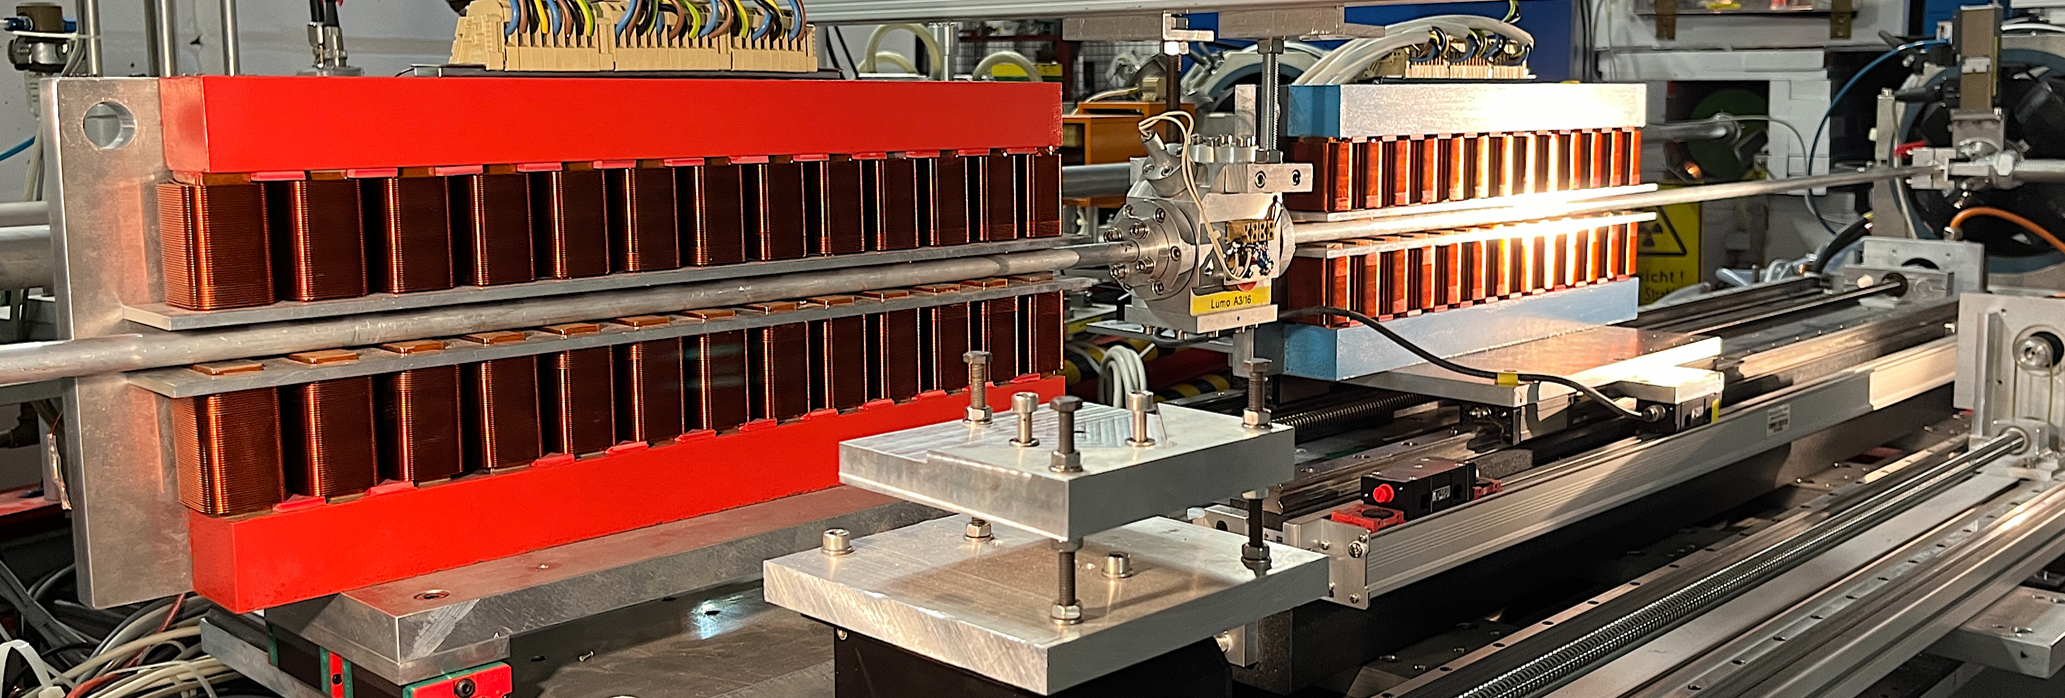
\includegraphics[width=\linewidth]{image/3-undulator.png}\\
  \caption[アンジュレータ]{測定に用いた2台のアンジュレータ。上流側の赤色アンジュレータは固定されているのに対し、、
  下流側の青色アンジュレータはステージに取り付けらえており、825 mmの可動範囲で$z$軸方向に移動できる。2台のアンジュレータの設計は同一で、
  13個のコイルが等間隔かつ極性が交互に配置されている。磁場1周期すなわちコイル2個分の長さは80 mmで、全長は520 mmである。
  図の手前には磁場調整の際に用いるホールプローブ取り付け台が設置されている。} 
  \label{undulator}
\end{figure}
\subsubsection{磁場制御}
各コイルには電源ボックスから電流を供給する。電流値を調整することで正弦波状の磁場を発生させることができる。
磁場の調整の際には、マトリックス型のホールプローブによる磁場測定を行う。
ホールプローブは40$\times$40 mm$^2$の領域に16$\times$16個、合計256個のホール素子を持ち、磁場の3次元成分を測定する(図\ref{hall})。
\begin{figure}[H]
  \centering
  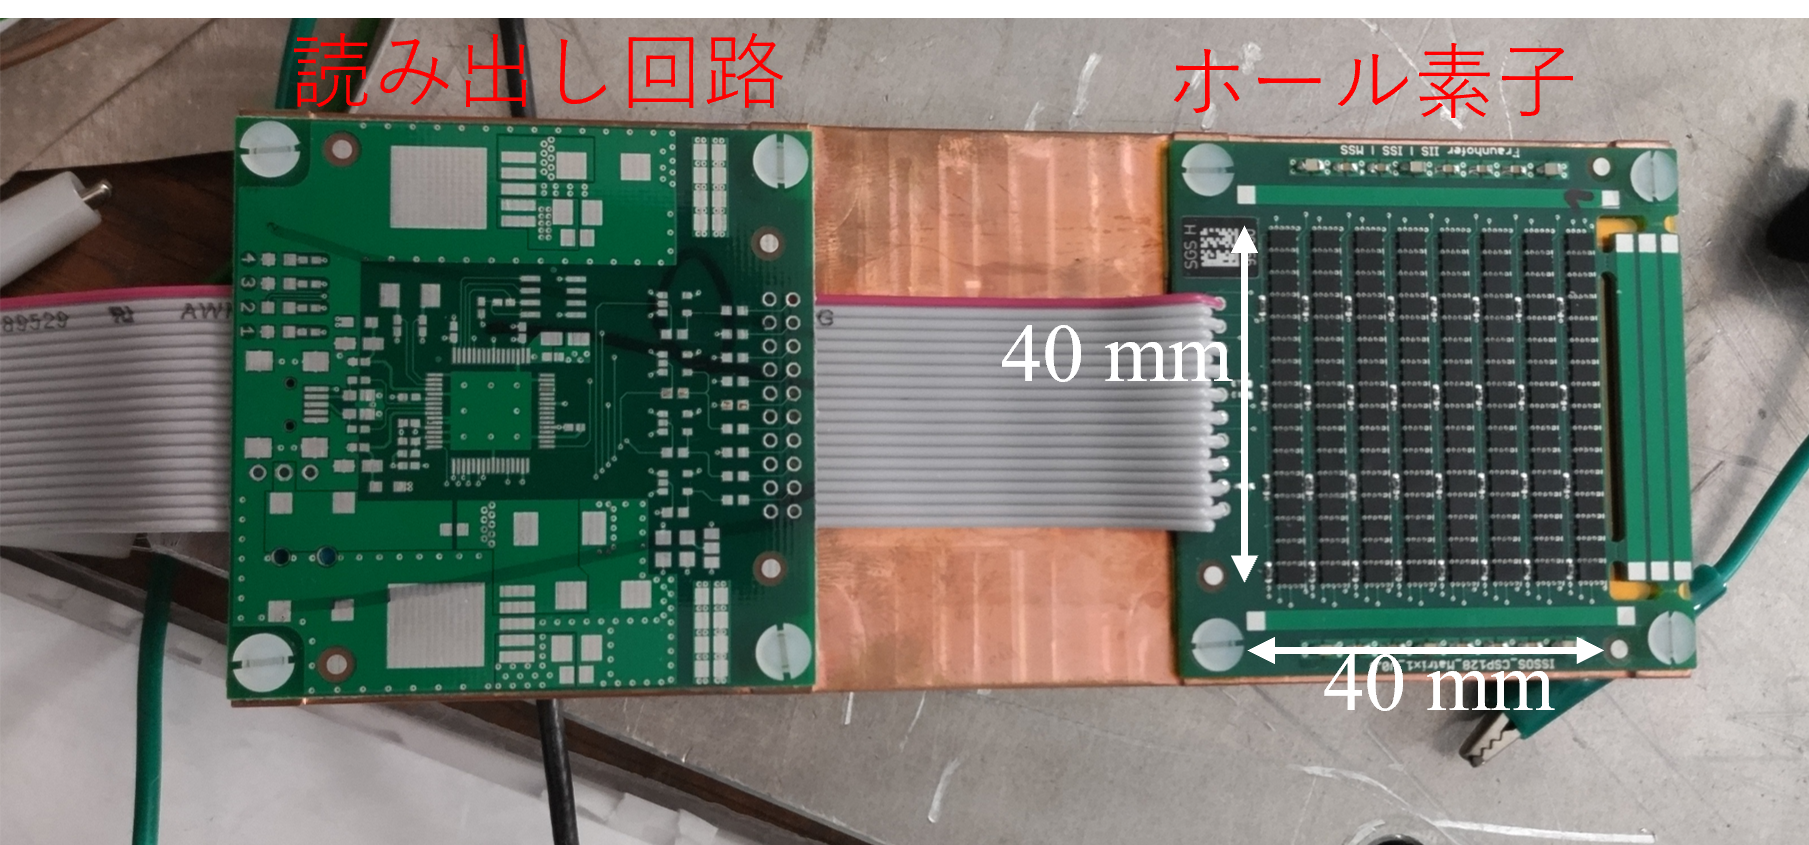
\includegraphics[width=0.7\linewidth]{image/3-hallmatrix.png}\\
  \caption[ホールプローブ]{マトリックス型のホールプローブ。40$\times$40 mm$^2$の領域に16$\times$16個、合計256個のホール素子を持ち、磁場の3次元成分を測定する。}
  \label{hall}
\end{figure}
ホールプローブはアンジュレータの中心を走査し磁場測定を行う。測定の様子を図\ref{hallscan}に示す。
\begin{figure}[H]
  \centering
  \includegraphics[width=0.8\linewidth]{image/3-HallMeasure.png}\\
  \caption[ホールプローブの走査]{ホールプローブによるアンジュレータの磁場測定の様子。ホールプローブはアンジュレータの中心を走査し、磁場の3次元成分を測定する。}
  \label{hallscan}
\end{figure}
アンジュレータ内の磁場は隣り合う複数の電磁石から影響を受けるため、適切な磁場を得るためには全ての電磁石の電流を同時に調整する必要がある。
ホールプローブによる測定と最適な電流値の決定を数回繰り返すことで、アンジュレータ内の磁場を調整する。
調整を止める基準として、アンジュレータを通過した後の電子軌道の変位が10~$\mu$m以下になることを定めて調整した。
調整後の磁場と、磁場の積分から計算される電子軌道の推定値を図\ref{fig:magnetic}に示す。
\begin{figure}[H]
  \centering
  \begin{subfigure}[h]{0.45\linewidth}
    \centering
    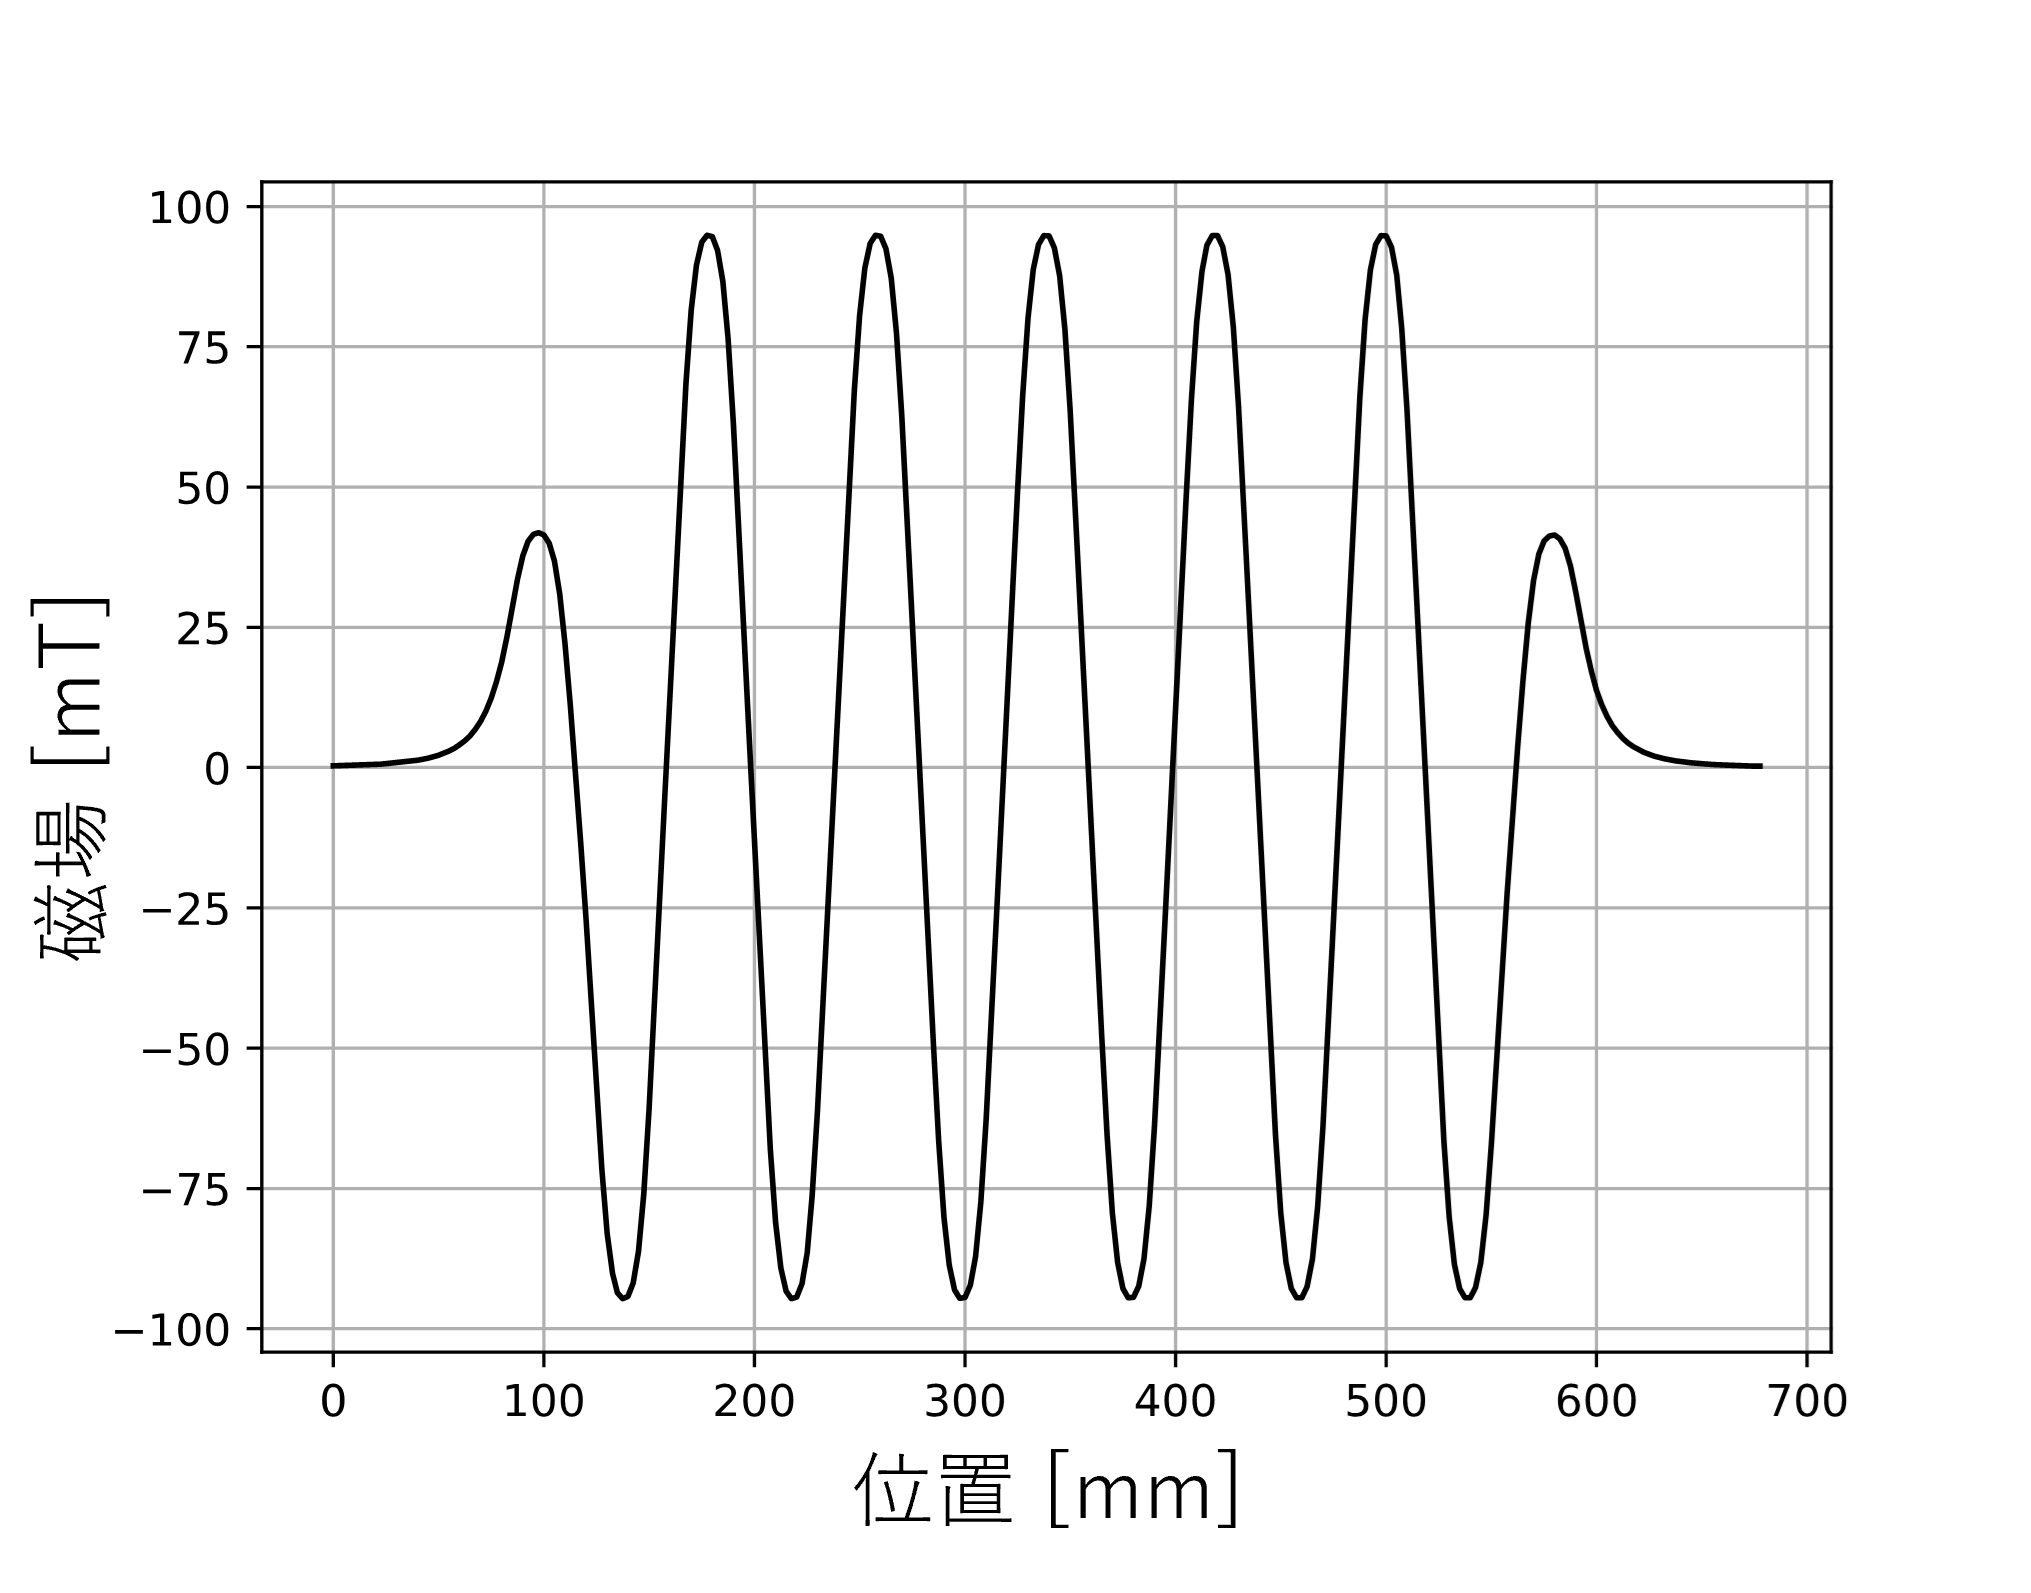
\includegraphics[width=\linewidth]{image/3-undulator_filed.png}
    \subcaption{磁場測定の結果}
  \end{subfigure}
  \hfill
  \begin{subfigure}[h]{0.45\linewidth}
    \centering
    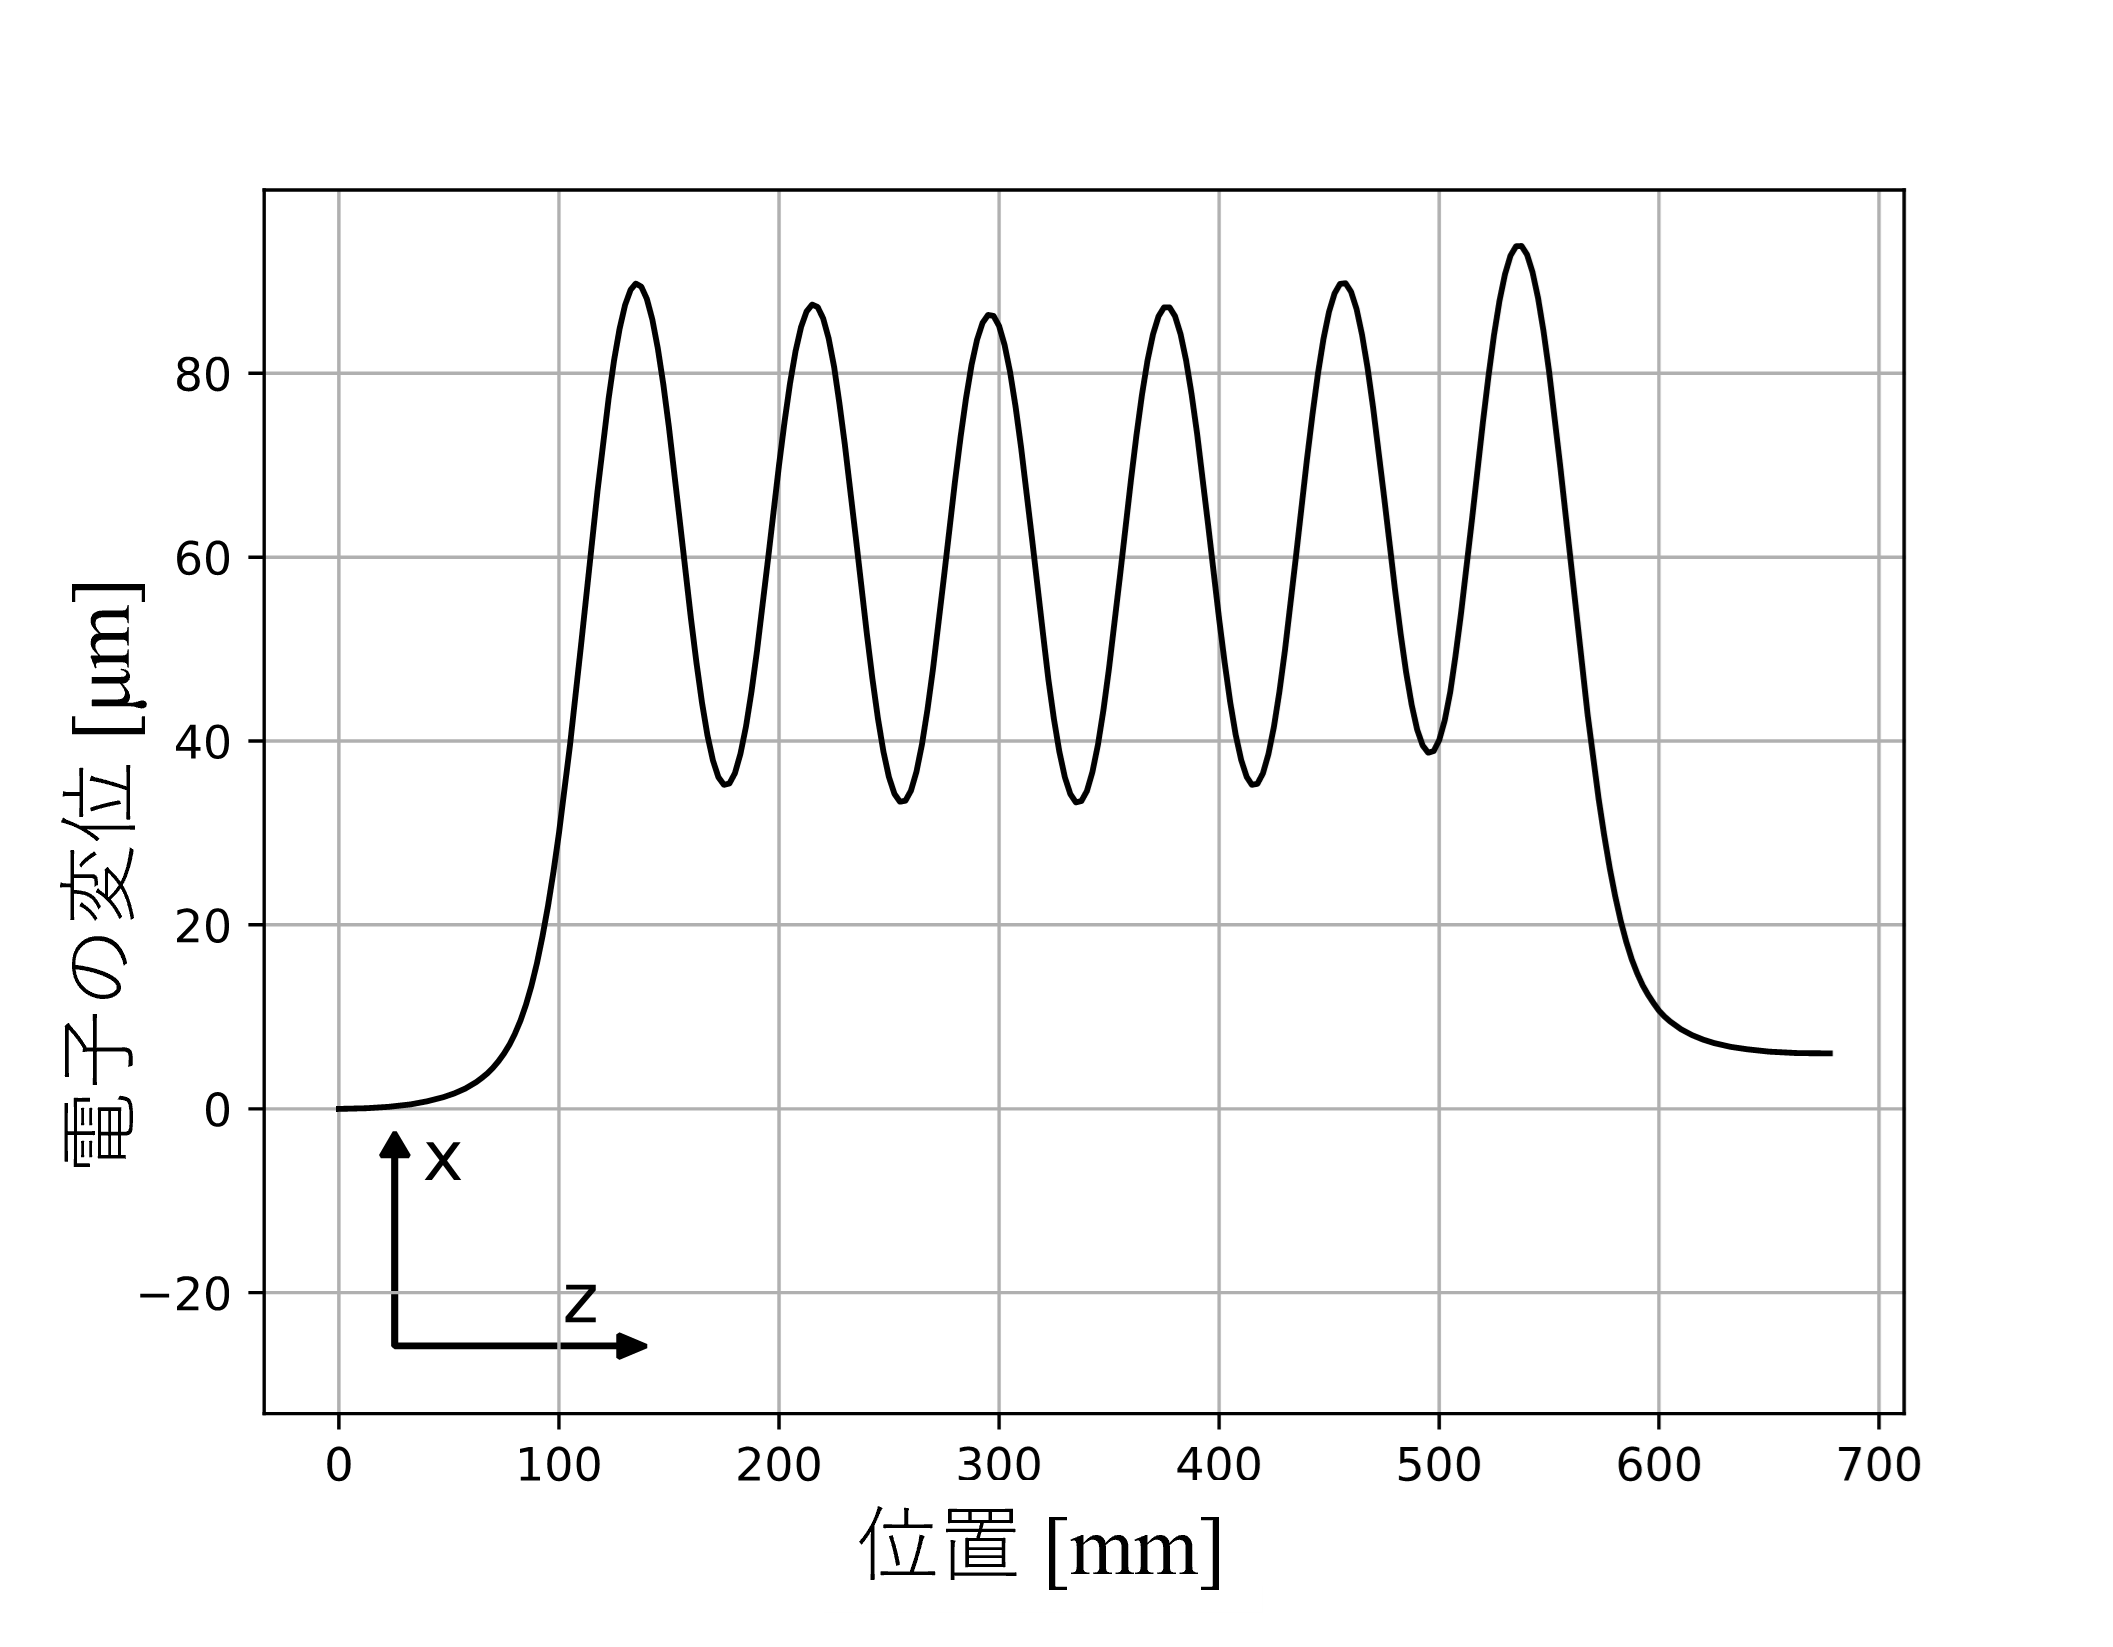
\includegraphics[width=\linewidth]{image/3-undulator_position.png}
    \subcaption{電子軌道の推定値}
  \end{subfigure}
  \caption[ホールプローブによる磁場測定の結果]{E = 180 MeVの時の磁場測定(B = 95~mT)の結果を示す。調整の結果、電子軌道の変位は10~$\mu$m以下に抑えられている。}
  \label{fig:magnetic}
\end{figure}
最後に、電子ビームエネルギーに対する目標磁場と偏向定数、および共鳴波長(放射光の共鳴波長=式(\ref{eq:resonance_wl}))を表\ref{undulator_setting}に示す。
\begin{table}[H]
  \centering
  \begin{tabular}{c|ccc}
    エネルギー [MeV]& 磁場設定値[mT]&偏向定数 $K$&共鳴波長 [nm]\\ \hline
    180 & 95  & 0.710 & 403.6\\
    195 & 130 & 0.971 & 404.2\\
    210 & 140 & 1.046 & 366.4\\
  \end{tabular}
  \caption[アンジュレータの磁場設定値]{アンジュレータの磁場設定値と偏向定数および共鳴波長(放射光のピーク波長)。
  180 MeVおよび195 MeVでは較正波長の404 nmと共鳴波長がほぼ一致したセットアップを実現できたが、210 MeVではアンジュレータのコイルの過電流を避けるために
  共鳴波長を短くする必要があった。}\label{undulator_setting}
\end{table}

\subsubsection{位置制御と読み取り}
アンジュレータは可動式ステージに取り付けられており、モーターによって移動させる。
可動範囲はビームライン上の制約から最大 825~mmに制限されており、間隔は通常の測定では 5 mmで指定する。
移動したアンジュレータの絶対値は、リニアエンコーダ(Heidenhain LC415)で 5 $\mu \text{m}$ の精度で読み出す。

\subsubsection{アラインメント}
セオドライトを用いてアンジュレータと較正用水銀灯、スリットの位置を調整した。セオドライトの基準は四重極電磁石(Q2, Q3)の中心で、この2点を通る直線をビームラインおよび光軸の基準としている。
アンジュレータの設置の際には、基準線をセオドライトを通して見ながら、アンジュレータの上流、下流側の磁石の中心を$x,y$方向に調整可能な調整ステージを動かして調整した。
%四重極電磁石はマーカーを基準に精密に水平に設置されていることが保証されている。
%~~よりも良い精度で水平に設置されている。

\subsection{分光光学系}
分光光学系全体の構成を図\ref{fig:optics}に示す。各素子間の長さは、素子の中心同士を結ぶ直線を測定した。
放射光の光軸が必ずしも素子の中心を通ることは保証されていないことと、放射光はスリットの大きさに対応して数~mm$^2$程度の広がりを持って入射するため、
実効的な距離は実測値と比較して最大10 mm程度のずれが生じると見積もった。
\begin{figure}[h]
  \centering
  \includegraphics[width=\linewidth]{image/3-optics.png}\\
  \caption[分光光学系の全体図]{分光光学系の全体図。光学素子間の長さの単位は mmである。}
  \label{fig:optics}
\end{figure}

\subsubsection{スリット}
矩形スリットを用いる。
スリット幅は4 mm($x$) x 6 mm($y$)であり、調節ねじにより上下、および左右のブレードが連動して動き、スリット幅を調整可能である。
これを$x$軸、$y$軸方向の可動ステージに乗せることでスリット全体の位置を0.1 mm単位で調整可能にした。

\subsubsection{回折格子}
回折格子はThorlab製の回折格子\cite{grating}を用いた。格子定数は1200/mm、大きさは50$\times$50~mm$^2$である。ピッチ・ヨー方向に調節可能な光学マウントによって固定され、さらに光学マウントが水平方向の回転ステージに設置されている。
これにより分光された放射光がカメラ方向に水平に反射されるよう調整できる。

\subsubsection{波長分散レンズ}
水平方向にのみ光波を収束するシリンドリカルレンズを用いた(図\ref{lens})。
大きさは40$\times$50~mm$^2$、焦点距離は1 m である。350 - 410 nmの波長領域に対してARコーティングが施されている。
このレンズもピッチ・ヨー方向および$y$軸方向の調節が可能な光学マウントによって固定される。
\begin{figure}[H]
  \centering
  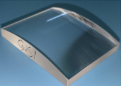
\includegraphics[width=0.4\linewidth]{image/3-lens.png}
  \caption[シリンドリカルレンズ]{シリンドリカルレンズ。水平方向のみに光波を収束し、垂直方向には窓として作用する。}
  \label{lens}
\end{figure}
水平墨出しレーザーの反射光を用いることでピッチ・ヨー回転の調整ができる。

\subsubsection{CMOS カメラ}
光学系は波長が400 nmの領域において動作するため、可視光領域のカメラを用いることができる。HAMAMATSU C14440-20UPを用いた。
仕様を以下に示す。
\begin{table}[h]
\centering
\begin{tabular}{c|c}
  ピクセル数 & 2304 $\times$ 2304\\
  ピクセルサイズ & 6.5 $\mu$m $\times$ 6.5 $\mu$m\\
  チップサイズ & 14.976 mm $\times$ 14.976 mm\\
  ビット深さ & 16 bit\\ 
\end{tabular}
\caption[CMOSカメラの仕様]{CMOSカメラ HAMAMATSU C14440-20UP の仕様}
\end{table}

\subsection{光学系のアラインメント}
青色レーザを用いて光学系全体の光軸調整を行った。青色レーザーの光軸はセオドライトを用いてビームライン中心と合わせる。
ビーム中心と合わせた青色レーザー光を光学系に通し、各光学素子の中心をとおるようにアラインメントを行う。
またレーザー墨出し器を用いて光学系全体の水平を確認する。回折格子とレンズの水平は青色レーザー光の位置を基準に調整した。
青色レーザーはミラーボックスの横20~cmの位置に設置され、次節で説明する水銀灯の較正にもミラーボックスを利用できるようモーターで横方向に移動可能である(図\ref{laser})。
\begin{figure}
  \centering
  \includegraphics[width=0.8\linewidth]{image/3-laser.png}\\
  \caption[青色レーザー]{青色レーザーと水銀灯用スリット。セオドライトを通してミラーボックスを目で見て、ビームライン中心にアラインメントした。}
  \label{laser}
\end{figure}
\section{データ取得}


\subsection{分光光学系の波長較正}
波長較正として水銀灯を用いる。
$400 \text{nm}$領域には2本の輝線があり、このスペクトルを光学系で観測することで2つの輝線スペクトルを観測できる。
水銀灯ランプはビームラインから垂直に5 mの位置に設置されており、ミラーボックス内のミラーを用いて電子ビームラインと同じ軌道を通って光学系に導かれる(図\ref{mirrorbox})。
ミラーボックスの直前には水銀灯用の円形スリットを設置した(図\ref{laser})。

輝線スペクトルをガウス関数でフィッティングし、中心位置のピクセルを対応する波長にする。
2本のスペクトル以外のピクセルは2本の輝線の波長 -ピクセル関係の線形性を仮定して決定する。
\subsection{データ取得}\label{sec:DAQ}
以下の手順を繰り返してデータ取得を行う。
ステージモータに指定する位置の値は0から825~mmの範囲で、5~mm間隔、計166点である。
\begin{itemize}
  \item アンジュレータのステージモータに次の指定位置の信号が送られる
  \item 指定の位置にアンジュレータが移動する
  \item カメラによる画像撮影の信号が4回送られる
  \item 画像撮影が完了し4枚の画像が追加されたことをDAQが確認する
\end{itemize}
同時にリニアエンコーダの位置読み出しも行い、データがラズベリーパイに保存される。この流れを図\ref{DAQ}に示す。
\begin{figure}
  \centering
  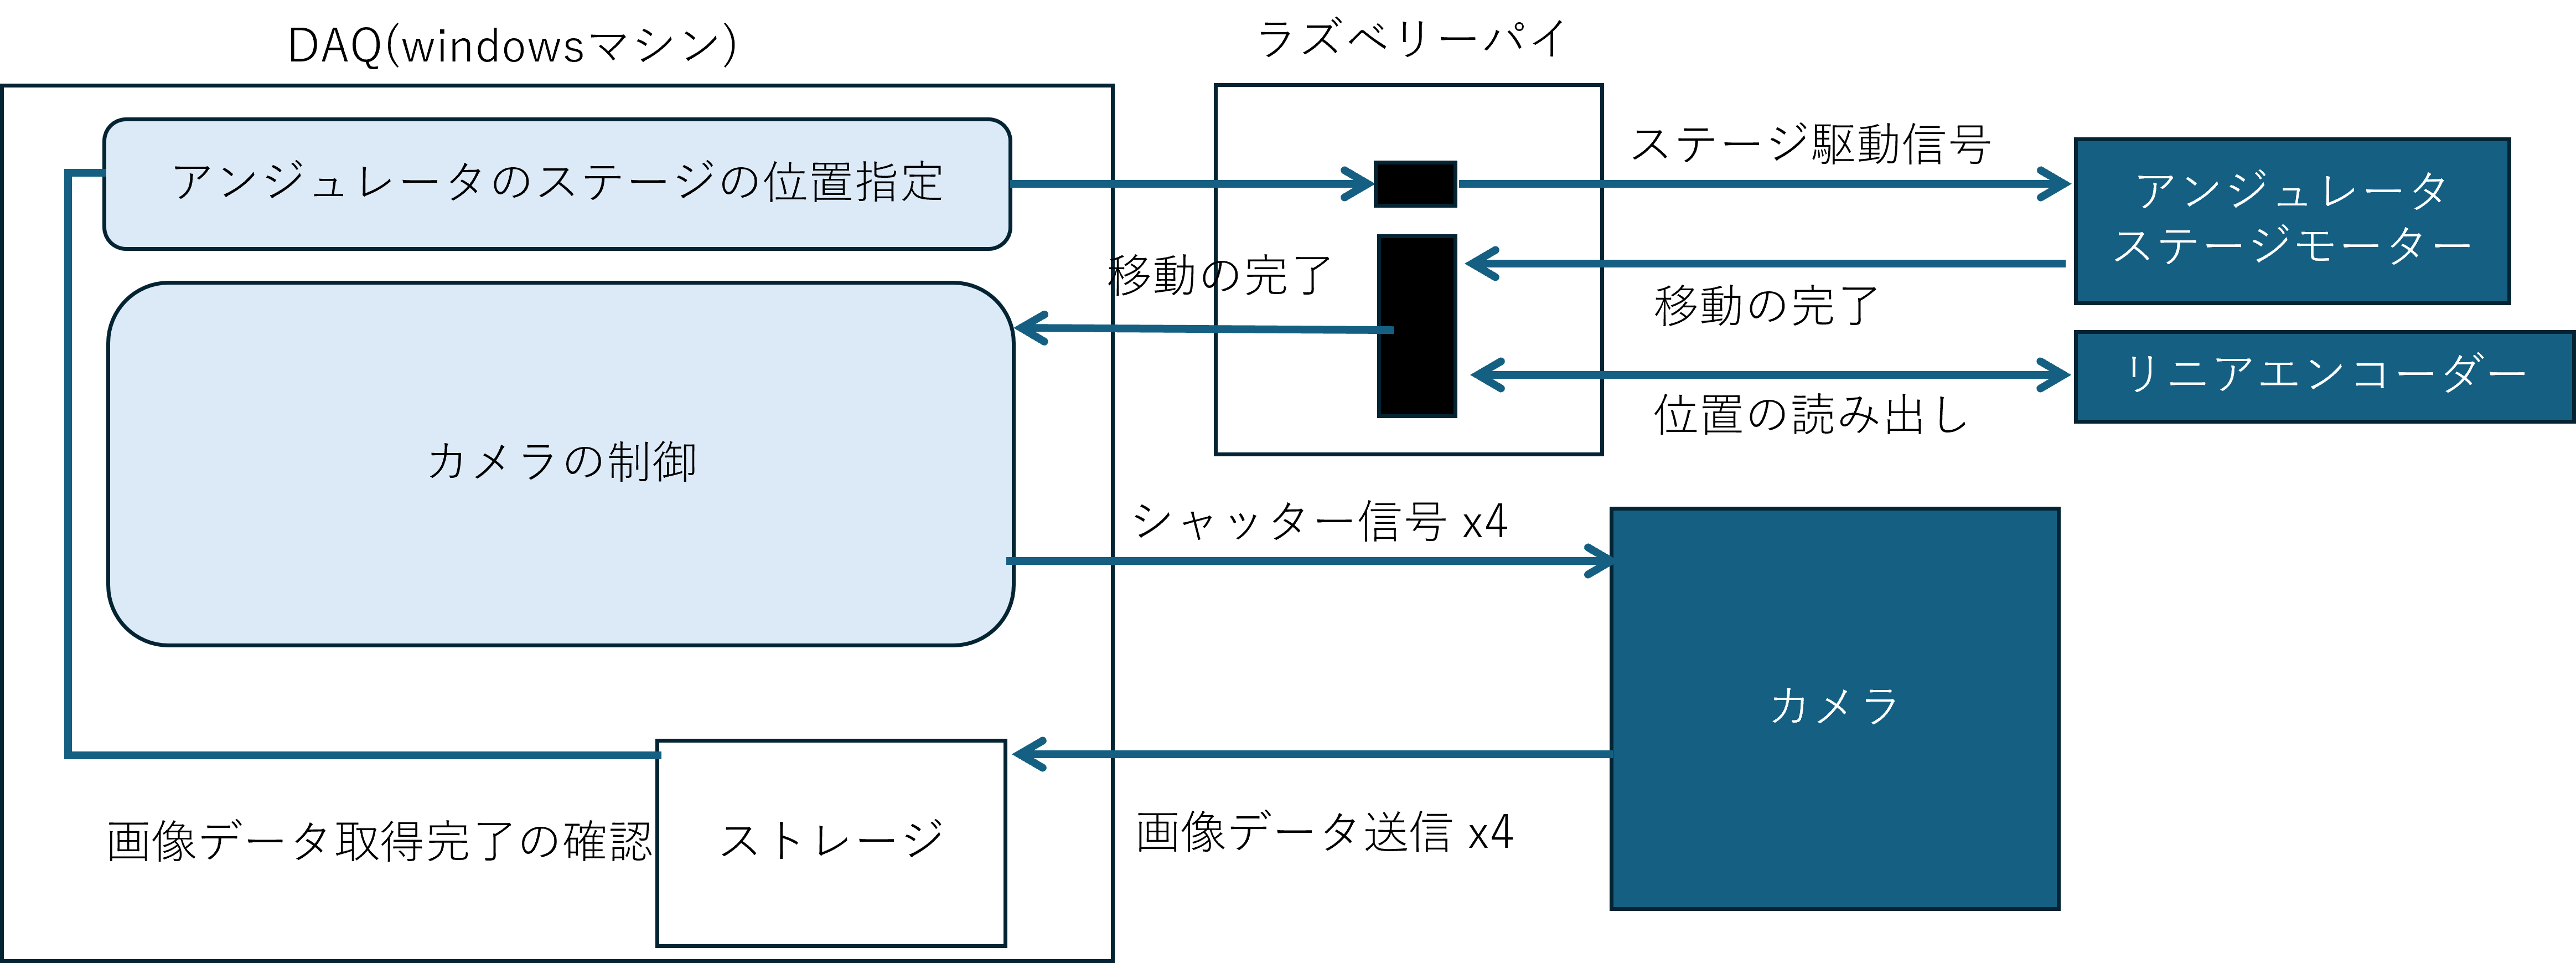
\includegraphics[width=0.8\linewidth]{image/3-DAQ.png}\\
  \caption[データ取得の流れ]{データ取得の流れ。アンジュレータが指定位置に移動するとカメラによる画像撮影が行われる。画像撮影が完了するとDAQに信号が送られ、次の指定位置にアンジュレータが移動する。
  ステージの移動が完了したらラズベリーパイからリニアエンコーダーに位置読み出しの信号が送信され、位置データがラズベリーパイへと送信される。これを166回繰り返すと1つのデータセットが取得できる。}
  \label{DAQ}
\end{figure}
\subsection{弾性散乱実験との同時運用における電子ビームエネルギー測定}

今回の実験の目的は弾性散乱実験における電子ビームエネルギーの精密測定である。この目的に照らし合わせて、弾性散乱実験でのデータ取得の前後にエネルギー測定を行うランプランを設定した(図\ref{beamtime})。
\begin{figure}
  \centering
  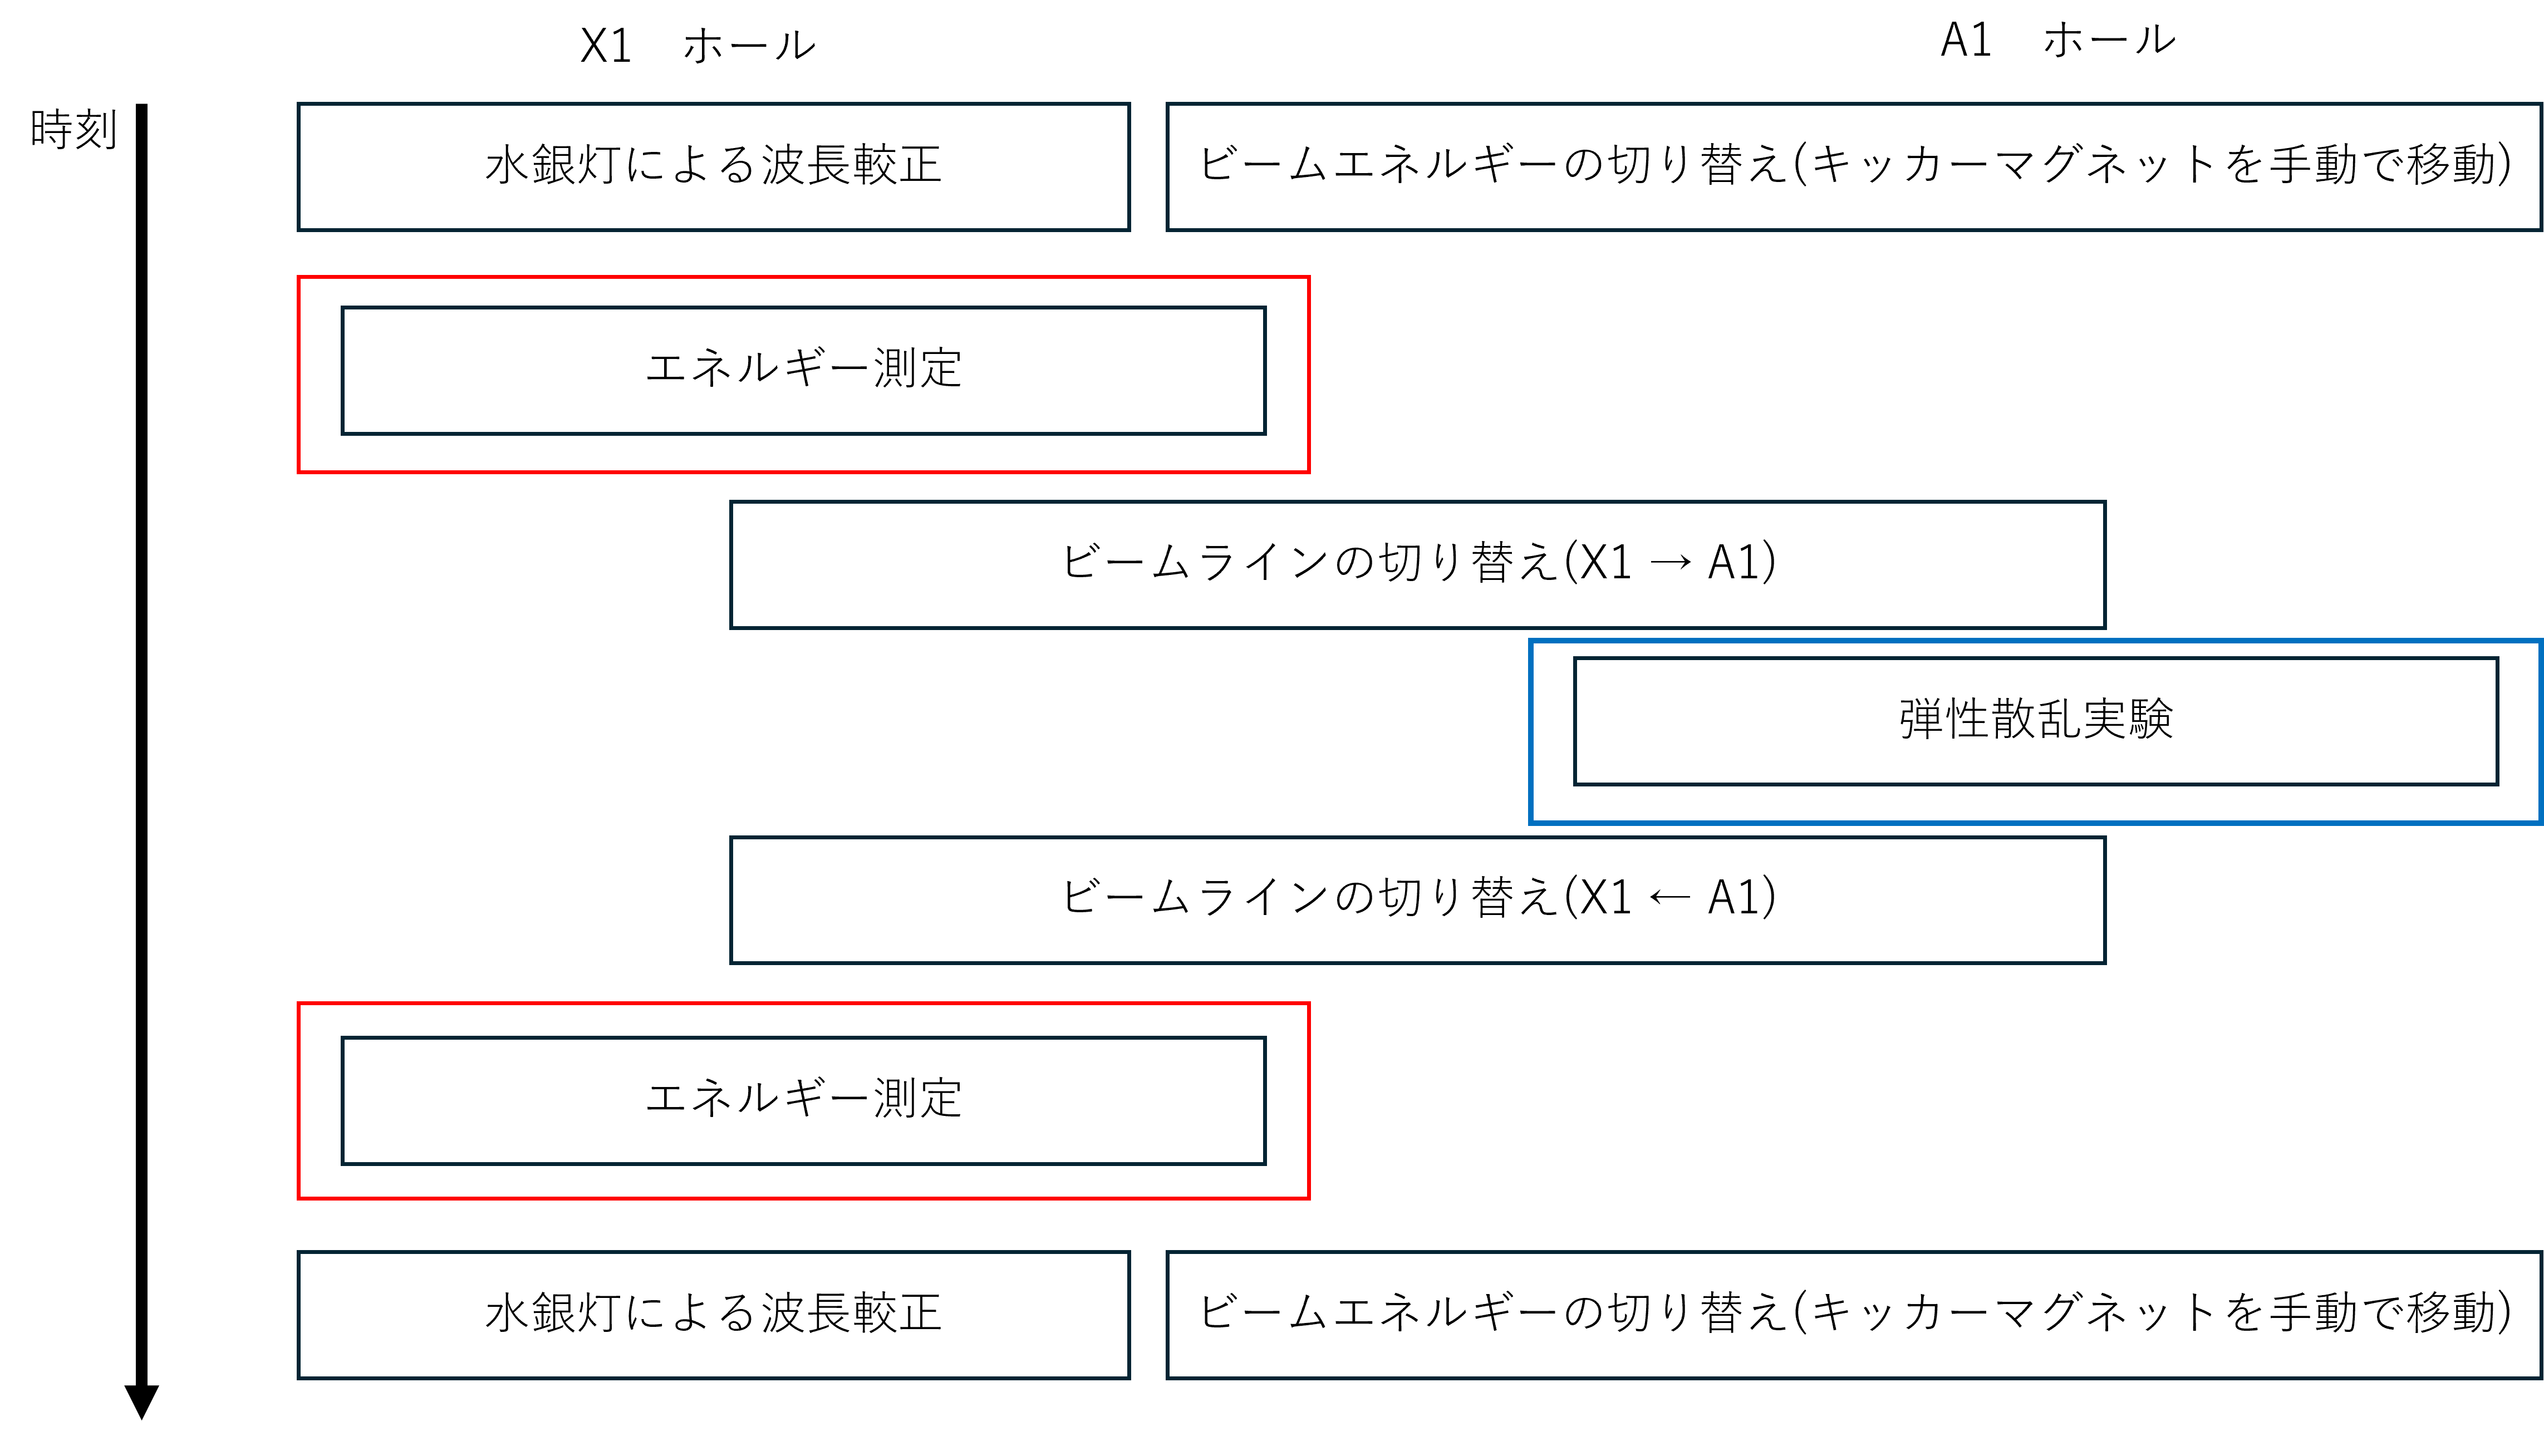
\includegraphics[width=\linewidth]{image/3-beamtime.png}\\
  \caption[弾性散乱実験とエネルギー測定の同時運用]{弾性散乱実験とエネルギー測定の同時運用。弾性散乱実験の前後にエネルギー測定を行う。赤、または青で枠の色がつけられている時間帯がビームが照射されている時間である。
  黒の枠で囲われた時間帯は、実験ホールでの作業と、一部ビーム調整の時間が含まれており、データ取得はできない。また「エネルギー測定」の内容は前節\ref{sec:DAQ}で述べたとおりである。}
  \label{beamtime}
\end{figure}
\subsection{下流側アンジュレータによるデータ測定}
パラメータ較正を目的として、下流側アンジュレータのみを用いたデータ取得を行う。
実験条件は$E_{beam} = 210$~MeVで、アンジュレータの磁場は140~mTとした。

上流のアンジュレータ(赤)はコイルに流す電流を0にしたうえで、残留磁場の影響を受けないように$x$軸方向に30~cmずらした。

\end{document}